\chapter{Experimental setup}

\intro{The \glsreset{lhc}\gls{lhc}, its preacceleator chain and experiments are described. An emphasis is given on the CMS experiment. The data recorded with it in 2012, 2015, and 2016 at 8 and 13~\TeV are used in this thesis.}

\section{Large Hadron Collider}

\subsection{Accelerator complex}

\myfigure{The accelerator complex at CERN. The figure is taken from~\cite{Mobs:2225847}.}{
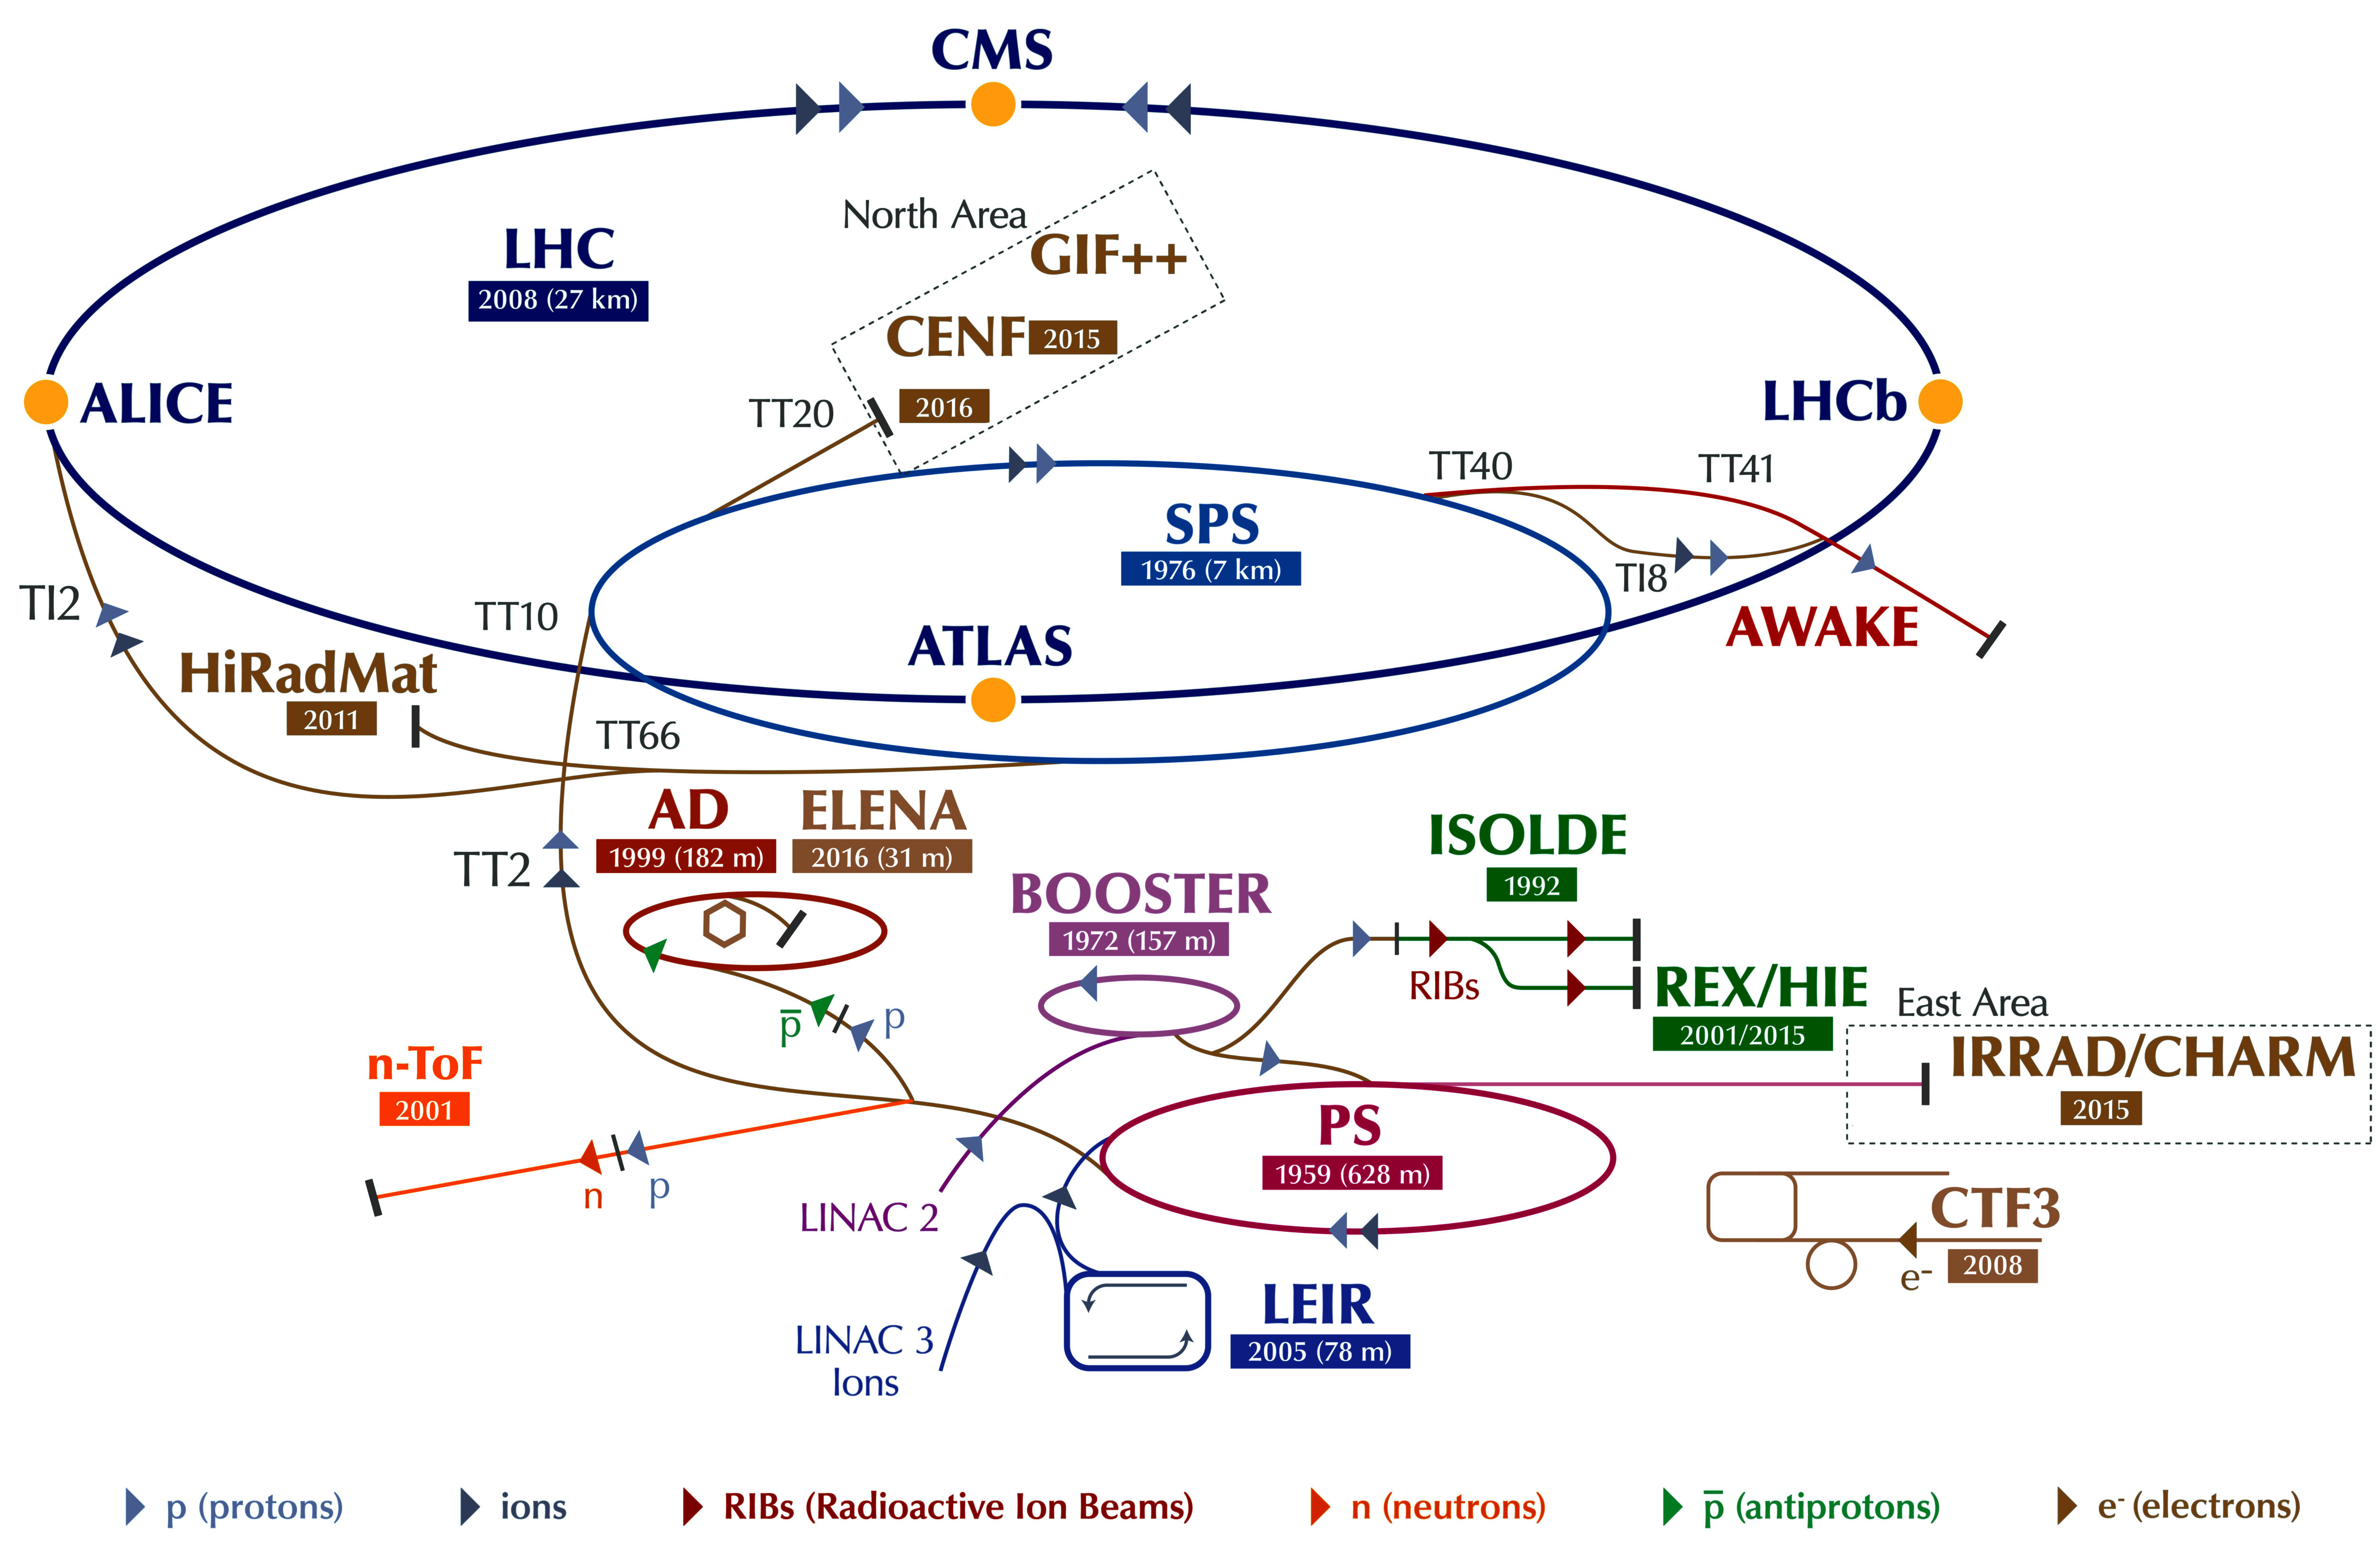
\includegraphics[width=0.99\textwidth]{figures/experiment/CERN_accelerator_complex.jpg}
}



momentum compaction

\subsection{Experiments}

\section{CMS experiment}

\subsection{Magnet}

\subsection{Tracker}

\cite{Chatrchyan:2014fea}

\subsection{Electromagnetic calorimeter}

\subsection{Hadronic calorimeter}

\subsection{Muon systems}
DT/RPC/CSC

\subsection{Data acquisition}
Trigger/DAQ

\subsection{Operations}
DCS/DSS
